% =========================================================================
% KBS 论文中文全文版(article + ctex 单栏中文排版,含全部 9 个附录)
% 编译:xelatex kbs_zh; bibtex kbs_zh; xelatex kbs_zh; xelatex kbs_zh
% =========================================================================
\documentclass[11pt,a4paper]{article}
\usepackage[UTF8]{ctex}
\usepackage[margin=1in]{geometry}
\usepackage{microtype}
\usepackage{graphicx}
\usepackage{booktabs}
\usepackage{amsmath,amssymb}
\usepackage{array}
\usepackage{makecell}
\usepackage{multirow}
\usepackage{xcolor}
\usepackage{enumitem}
\usepackage[numbers]{natbib}
\usepackage[hidelinks]{hyperref}
\usepackage{pifont}
\usepackage{xurl}
\DeclareUrlCommand\filep{\urlstyle{tt}}   % 文件路径用,正确处理下划线
\newcommand{\cmark}{\ding{51}}
\newcommand{\xmark}{\ding{55}}
\sloppy
\renewcommand{\arraystretch}{1.15}
\newcommand{\qtype}[1]{\texttt{\small #1}}
\newcommand{\op}[1]{\textsc{\small #1}}

\title{\bfseries 超越 Top-K:面向知识图谱问答中\\答案几何失配的类型化算子族}
\author{作者姓名\\ \small 单位,中国}
\date{}

\begin{document}
\maketitle

\begin{abstract}
\noindent
GraphRAG 系统正趋向于日益精巧的 top-$K$ 检索算法——社区摘要、个性化 PageRank、LLM 路径模板、束搜索——但 top-$K$ 内嵌了一个关于\emph{答案几何}的隐含假设:即答案是一个可按表面相关性排序的小集合。出于\emph{信息论}而非模型能力的原因,该假设在工业级知识图谱常见的三类可计算模式上系统性失效:无界枚举、多约束求交、求补/非成员。我们把这一现象命名为\textbf{答案几何失配},并论证它类比于数据库中的 OLTP/OLAP 之分:B 树索引擅长点查询,却在聚合查询上结构性地错误,无论如何调优。我们提出 \textbf{Strategy-Routed GraphRAG},一套由六个类型化检索算子(\op{lookup}、\op{exhaustive}、\op{complement}、\op{path-plan}、\op{constrained-join}、\op{dual-subgraph})构成的算子族,每个算子均被\emph{推导}为满足其目标类信息需求的原语(其中四个算子在本基准上承重,另两个依推导保留);分发器是一个轻量 LLM 查表。一次预言机消融把全部增益定位到算子上(预言机 88.2\% vs LLM 分发 88.6\%,$\Delta\!=\!-0.4$ 个百分点)——\textbf{这是一篇关于算子、而非分类器的论文}。在我们公开发布、专为暴露答案几何失配而设计的双语基准 \textbf{RadarKG-QA-499} 上(计数题中位基数是公开基准的 $3.4$ 倍),该算子族达到 \textbf{88.6\%},而基线为 52.7\%、零样本路径规划器为 60.3\%($+35.9$ / $+28.3$ 个百分点,配对自助置信区间严格为正,对 $K{=}8{\to}20$ 稳健)。跨域到 KQA Pro,类型学与分发器无需重训即可迁移(67.4\% 路由匹配;\op{dual-subgraph} 在 SelectBetween 上 $+11$ 个百分点);绝对增益随基准中答案几何失配的占比而变——公开基准系统性地欠采样了这一区间,我们将其作为社区空缺加以记录。单次查询成本 \$0.00041(每准确率点 \$0.00084),该算子族可用于工业级 KGQA 部署。
\end{abstract}

\noindent\textbf{关键词:} 知识图谱问答;图检索增强生成;类型化检索算子;大语言模型;知识驱动决策支持

% =========================================================================
\section{引言}
\label{sec:intro}

\paragraph{现象。}
GraphRAG 的工业部署 \citep{edge2024graphrag,gutierrez2024hipporag,luo2024rog,sun2024tog,ma2025tog2} 面临一类顽固的查询分布,统一施加的 top-$K$ 检索无法回答。考虑雷达知识图谱上的三个自然问题:

\begin{table}[h]
\centering\small
\begin{tabular}{p{0.43\linewidth}|p{0.49\linewidth}}
\toprule
\textbf{问题形态} & \textbf{为何 top-$K$ 失效} \\
\midrule
\emph{"美国列装了多少部雷达?"} & 答案集合含 $>$400 个元素;受检索预算约束的任何 $K$ 都无法枚举它。 \\
\emph{"由美国厂商研制\textbf{且}工作于 S 波段的雷达。"} & top-$K$ 无法跨约束表达\emph{交集}。 \\
\emph{"AN/TPY-2 是否出口到日本?"} & 知识图谱宣告"存在"而非"不存在";top-$K$ 漏掉非局部的否定。 \\
\bottomrule
\end{tabular}
\end{table}

这些并非 LLM 的失败:无论模型能力多强,$K{=}8$ 时 top-$K$ 无法枚举 400 个答案、无法跨两个独立排序信号表达"与"、也无法在只存"存在"的知识图谱中宣告"不存在"。它们是\emph{信息论意义}上的失败——检索到的集合缺少任何下游推理器所需的比特。在 RadarKG-QA-499(\S\ref{sec:benchmark})中,约 30\% 的自然问题落入这些类别;无论 LLM 选型或 $K \in \{8, 20\}$,基线 top-$K$ 在其上仅得 4--12\%(\S\ref{sec:rq1},表~\ref{tab:k20})。

\paragraph{诊断:答案几何失配。}
top-$K$ 内嵌了一个关于\emph{答案几何}的隐含假设——答案是一个可按对查询的表面相关性排序的小集合。该假设对事实型查询成立(WebQSP 与 NaturalQuestions 的典型评测区间),但在工业级知识图谱常见的三类可计算模式上失效:
\begin{itemize}[topsep=0pt,itemsep=0pt,leftmargin=*]
  \item \textbf{无界枚举}(计数、列举):信息需求是\emph{完整集合};top-$K$ 受 $K$ 约束。
  \item \textbf{多约束求交}(跨独立排序信号的"与"):信息需求是\emph{集合交集};top-$K$ 的排序混淆了各约束。
  \item \textbf{求补/非成员}(确认"不存在"):信息需求是\emph{全局否定};知识图谱只存正三元组,故"不存在"不出现在任何局部窗口中。
\end{itemize}
我们称之为\textbf{答案几何失配}(AGM):查询的信息需求与 top-$K$ 几何所能交付者结构性地不相容。某基准中 AGM 占 30\% 还是 5\%,是\emph{基准分布}的属性,而非 top-$K$ 自身的属性——公开基准系统性地欠采样该区间(\S\ref{sec:bench-design},表~\ref{tab:bench-distribution}),而工业级知识图谱系统性地过采样它。

\paragraph{洞见:让信息需求匹配算子。}
这一模式在数据库理论中并不陌生。B 树索引擅长点查询(\texttt{SELECT WHERE id\!=\!5}),却是聚合查询(\texttt{COUNT(*) GROUP BY country})结构上不当的执行计划——不是因为 B 树差,而是因为查询的信息需求需要不同的访问模式。数据库的应对不是改进 B 树,而是增加\emph{类型化执行计划}(哈希连接、全表扫描、排序归并)及一个挑选正确计划的查询优化器。\textbf{top-$K$ 就是 GraphRAG 的 B 树}:对事实检索最优,对分析型 KGQA 结构失配。修复之道不是更好的排序器,而是\emph{为每个查询的信息需求配上正确的算子}。我们枚举 top-$K$ 无法满足的信息需求类别,并推导出一套六算子的类型化算子族(\S\ref{sec:method})。一个轻量 LLM 分发器把每个问题映射到其算子类。

\paragraph{系统(以及预言机意外)。}
我们把该框架实例化为 \textbf{Strategy-Routed GraphRAG}:一个 LLM 分发器 + 六个类型化算子 + 一个读取算子证据的 LLM 作答器。分发器零样本即达 93\% 的类型分类准确率——但其准确率并非承重。\textbf{一次以金标问题类型路由替换 LLM 分发器的预言机消融,端到端达到 88.2\%,对 LLM 分发器的 88.6\%($\Delta\!=\!-0.4$ 个百分点;\S\ref{sec:rq3})}:对基线 $+35.9$ 个百分点的全部增益是算子驱动而非分发器驱动的。\textbf{这是一篇关于算子、而非分类器的论文。} 分发器是一个 LLM 恰好能很好求解的 $O(1)$ 查表;分析性贡献在于满足 top-$K$ 无法满足之信息需求的算子族。

\paragraph{贡献。}
我们的贡献主要是\emph{概念性}的,而非工程性的:价值在于诊断与"类型学$\to$原语"对应关系,而非任一算子的精巧(\op{exhaustive} 即"不截断",\op{complement} 即"枚举后取反")。具体地:
\textbf{(1)} \textbf{答案几何失配诊断}:一个根植于信息论下界的精确论述,说明 top-$K$ 检索在 KGQA 上何时、为何系统性失效,并借数据库理论的 OLTP/OLAP 类比加以框定——可迁移到雷达领域之外。
\textbf{(2)} \textbf{一种"类型$\to$原语"对应关系}:我们识别出 top-$K$ 无法满足的信息需求类别,并证明每一类一对一地映射到一个\emph{可计算}的图访问原语,由此得到一套六算子。科学主张是这一映射(哪类需要哪种访问模式、为什么),而非算子工程;与此一致,预言机消融表明分发器贡献约 0 个百分点——增益来自\emph{拥有正确的原语},而非分类得好(其中三个算子在本基准上承重;\S\ref{sec:rq2})。
\textbf{(3)} \textbf{RadarKG-QA-499},首个为暴露 AGM 而显式设计的 KGQA 基准(计数题中位基数是公开基准的 $3.4$ 倍),并含一个 26 题的分布外双语压力子集。
\textbf{(4)} \textbf{实证}:在全部 499 题上对基线 $+35.9$ 个百分点、对单策略路径规划 $+28.3$ 个百分点,配有配对自助置信区间与多项消融(检索预算、逐算子、算子族规模、预言机分发器、跨域),把增益定位到算子设计。
此外我们报告一个方法学观察——对双语/别名组件的分布内评估会产生假阴性消融(分布外集上出现 0 $\to$ $+11.5$ 个百分点的差距;\S\ref{sec:rq3})——鉴于其置信区间处于边界,我们将其作为多语 KGQA 评估的一个注意事项,而非主要主张。

% =========================================================================
\section{方法}
\label{sec:method}

\subsection{流水线}
一个问题经三个 LLM 阶段处理——\textbf{分发器}(选择算子)、\textbf{解析器}(抽取实体与关系链)、\textbf{作答器}(把证据渲染为自然语言答案)——及一个仅查图谱的\textbf{执行器}(图~\ref{fig:pipeline})。知识图谱(RadarKG-v2:16\,513 条三元组、98 种关系+属性、4\,827 个实体)只在执行器中被查询,绝不经由 LLM。

\begin{figure}[h]
\centering
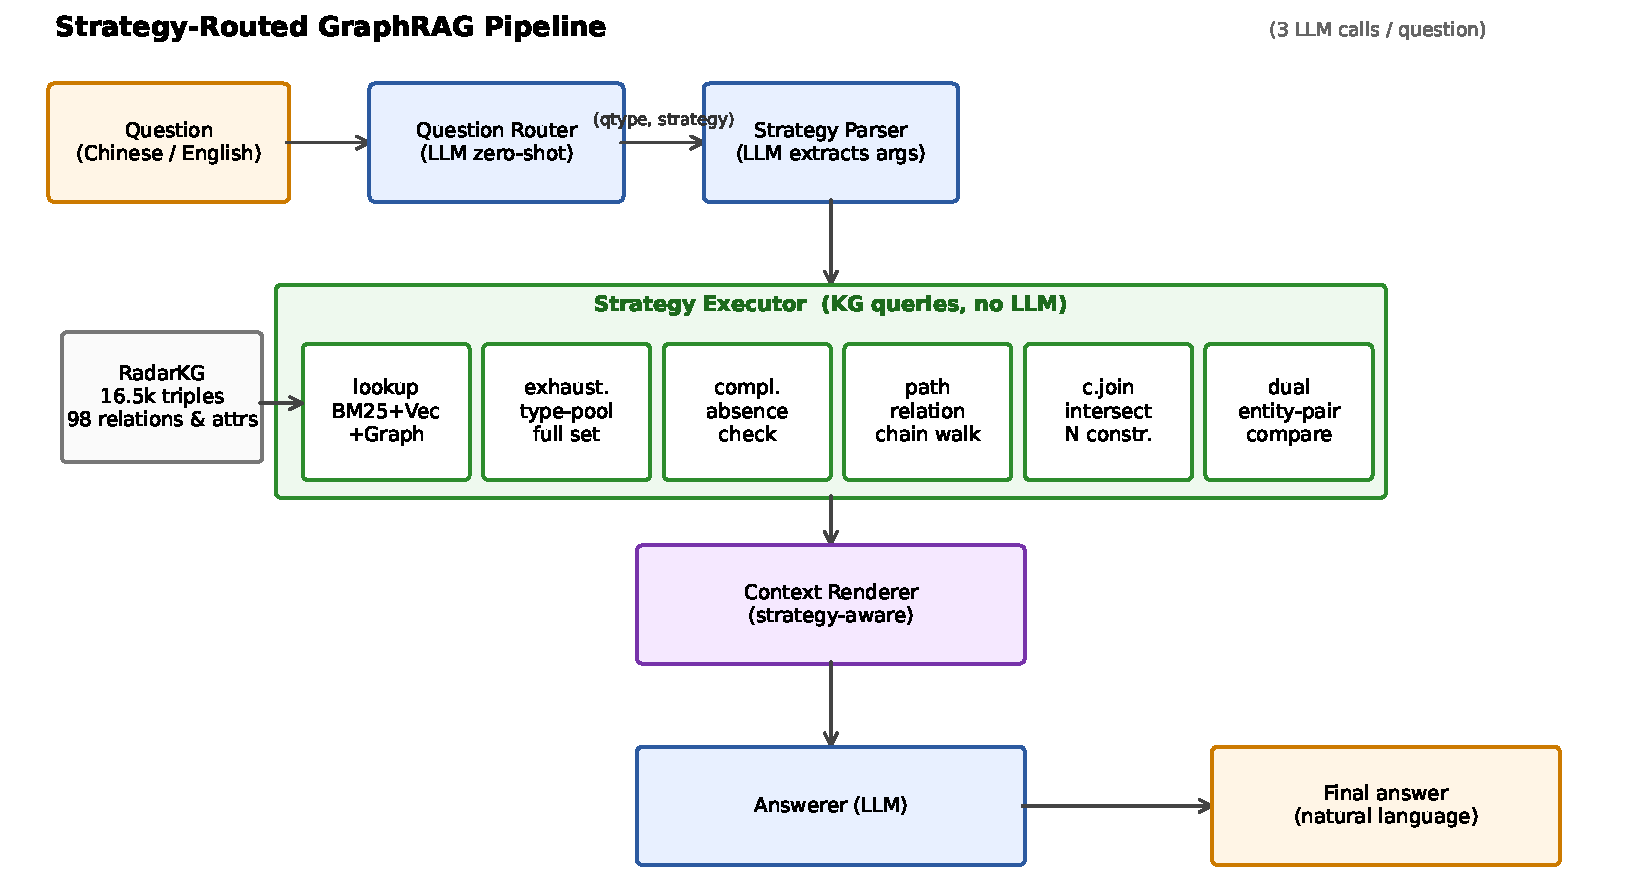
\includegraphics[width=0.95\linewidth]{figures/fig1_pipeline.pdf}
\caption{Strategy-Routed GraphRAG 流水线。}
\label{fig:pipeline}
\end{figure}

\subsection{问题类型学}
我们定义 11 种问题类型,植根于各自所需的\emph{检索模式}(而非表面形式)。每种类型确定性地映射到一个算子。

\begin{table}[h]
\centering\small
\caption{11 类类型学 $\to$ 6 算子映射。}
\label{tab:typology}
\begin{tabular}{p{0.35\linewidth} p{0.27\linewidth} l}
\toprule
\textbf{类型} & \textbf{信号} & \textbf{算子} \\
\midrule
\qtype{single\_hop}                                                 & 实体+属性     & \op{lookup} \\
\qtype{relation\_inverse,} \qtype{agg\_count,} \qtype{agg\_enum}    & 无界枚举      & \op{exhaustive} \\
\qtype{two\_hop\_bridge,} \qtype{three\_hop\_chain}                 & 组合 $k\!\geq\!2$ & \op{path-plan} \\
\qtype{attr\_filter}                                                & 约束之"与"    & \op{constrained-join} \\
\qtype{negation,} \qtype{unanswerable}                              & 不存在        & \op{complement} \\
\qtype{set\_compare}                                                & 两实体        & \op{dual-subgraph} \\
\qtype{distractor}                                                  & 消歧          & \op{lookup} \\
\bottomrule
\end{tabular}
\end{table}

\subsection{从信息需求推导算子族}
\label{sec:derivation}

我们不靠观察常见失败模式来挑选算子,而是枚举 top-$K$ 无法满足的\emph{信息需求类别},为每一类推导一个算子,再为 top-$K$ \emph{确能}满足的那一类补上 \op{lookup}。表~\ref{tab:reqs} 把推导显式化;表~\ref{tab:operators} 给出实现机制。

\begin{table*}[t]
\centering\small
\caption{算子族的信息需求推导。每一行依据满足其需求的最小访问模式确定其算子;top-$K$ 在每一行因不同原因失效。}
\label{tab:reqs}
\setlength{\tabcolsep}{4pt}
\begin{tabular}{p{0.16\linewidth} p{0.27\linewidth} p{0.28\linewidth} p{0.20\linewidth}}
\toprule
\textbf{模式} & \textbf{信息需求(最小)} & \textbf{为何 top-$K$ 失效} & \textbf{推导出的算子} \\
\midrule
身份/事实型     & 单条最佳匹配三元组                       & (无——top-$K$ 即可满足)                       & \op{lookup} = BM25 $\oplus$ 向量 $\oplus$ RRF \\
无界枚举        & 某关系的\emph{完整}头/尾集合             & $K$ 是上界,而答案集合不是                     & \op{exhaustive} = $\{h \mid (h,r,t)\!\in\!\text{KG}\}$ \\
多约束"与"      & $N$ 个关系头集合的交集                    & 排序无法表达"与",会混淆信号                   & \op{constrained-join} = $\bigcap_i \text{heads}(r_i,t_i)$ \\
求补/不存在     & 完整的\emph{已知}集合,再显式给出缺口      & 知识图谱只存正事实,"不存在"是非局部的         & \op{complement} = 先枚举再核验 \\
组合 $(k\!\geq\!2)$ & 跨 $k$ 个关系、保留跳数结构的路径    & top-$K$ 是扁平的,会丢失跳边界                 & \op{path-plan} = $\text{tails}_{r_1}\!\circ\!\dots\!\circ\!\text{tails}_{r_k}$ \\
二元比较        & \emph{双方}子图均显式且对齐              & top-$K$ 可能饿死一方,且无法对齐               & \op{dual-subgraph} = 并行 $\text{tails}(A,B)$ + 集合运算 \\
\bottomrule
\end{tabular}
\end{table*}

每个算子都是满足其所在行信息需求的\emph{最小}访问模式:从 \op{exhaustive} 中去掉"穷举"会重新引入 $K$ 受限的失败;从 \op{constrained-join} 中去掉交集会恢复排序混淆的失败;以此类推。该推导既论证了算子族的\emph{数目}(六个需求类别、六个算子),也论证了其\emph{内容}——二者都不是经验性的曲线拟合。经验性问题在于实践中是否存在\emph{额外}类别;\S\ref{sec:rq2} 的算子族规模消融回答了这一点(三个承重算子在互不相交的题目切片上具有可加贡献;在本基准上一个 4 算子子集即可匹配完整 6 算子的准确率)。

\paragraph{推导主张的范围。}
上述框架\emph{植根于}把信息需求匹配到访问模式;我们并不主张\emph{形式完备性}。这六类需求是通过考察我们雷达基准上常见的 KGQA 失败模式识别出来的,并非一个封闭分类:更多模式——聚合算术(对数值属性求 \texttt{SUM}、\texttt{AVG})、传递闭包、时间区间约束、模糊匹配——会催生额外算子(讨论 \S\ref{sec:discussion} 勾勒了扩展路径)。该推导给了算子族一个有原则的\emph{来源},但并非任何代数意义上\emph{极小性}或\emph{覆盖性}的证明。

\begin{table*}[t]
\centering\small
\caption{六算子族——实现机制。}
\label{tab:operators}
\begin{tabular}{l p{0.78\linewidth}}
\toprule
\textbf{算子} & \textbf{机制} \\
\midrule
\op{lookup}            & BM25 + 双编码器 + RRF + 2 跳图扩展;对解析器抽取出的参数,(头, 关系)经知识图谱直查旁路。 \\
\op{exhaustive}        & $\{h \mid (h, r, t) \in \text{KG}\}$,无 $K$ 截断。空结果时启用等价类回退(见下)。 \\
\op{complement}        & 枚举 $\{t \mid (h, r, t) \in \text{KG}\}$;标记空集/非成员,使 LLM 显式输出"否"而非臆造。 \\
\op{path-plan}         & 带逆向遍历 $r^{-1}$ 的关系链 BFS,返回终点实体与完整边轨迹。 \\
\op{constrained-join}  & 跨 $N$ 个约束的头集合求交,带\textbf{等价类回退}:交集为空时合并语义等价关系(如 \texttt{countryOfOrigin}\,$\cup$\,\texttt{operatedBy})——化解多源抽取带来的子图不相交噪声。 \\
\op{dual-subgraph}     & 在 $(A,B)$ 上对共享关系并行执行 \textit{tails\_of},并排渲染,预先算好 $A\!\cap\!B$、$A{\setminus}B$、$B{\setminus}A$。 \\
\bottomrule
\end{tabular}
\end{table*}

\op{lookup} 算子还充当分发器错误的安全回退:被误路由的问题会退化为标准混合检索,而非退化为某个错误算子的空结果。

\paragraph{关于等价类回退(一处语义警示)。}
\op{constrained-join} 的回退会合并语义\emph{相关但不相同}的关系——如 \texttt{countryOfOrigin}(在哪国建造)与 \texttt{operatedBy}(谁列装),二者对出口装备并不相同。为防止其悄悄抬高准确率,该回退被设了门槛:\emph{仅}在严格交集为空时触发,且基准金标由\emph{严格}关系算出(附录~\ref{app:kg}),绝不取并集。因此对严格答案集非空的问题,回退不会触发;当它确实触发时(系统侧因解析/别名失配致交集为空),只会引入严格金标判为假阳的候选——只会扣分、不会抬分。我们直接量化(执行器级、对金标精确集匹配):回退仅在 \textbf{50 道 \qtype{attr\_filter} 中的 2 道}上触发,关掉它使 \qtype{attr\_filter} 准确率改变 \textbf{$0.0$ 个百分点}——那两道的严格交集为空,是因为并集也无法解决的取值形态不匹配。故 $+80$ 个百分点的增益\emph{并非}关系放宽的产物,它来自 \op{constrained-join} 表达了 top-$K$ 排序所混淆的交集。

\subsection{分发器与双语别名层}
一个带类型学定义 + 5 个示例的零样本 DeepSeek-Chat 路由器把问题 $\to$ 类型 $\to$ 算子。路由准确率 93.0\%。一个贯穿全局的\textbf{双语别名层}(五级级联:直接匹配 $\to$ 614 形态别名索引 $\to$ 频段归一 $\to$ 后缀剥离 $\to$ 等价类合并)处理取值为中英混合的工业级中文知识图谱。

% =========================================================================
\section{基准:RadarKG-QA-499}
\label{sec:benchmark}

\subsection{知识图谱}
RadarKG-v2 含 4\,827 个实体、12\,219 条实体间边,外加约 80 种类型化属性(共 16\,513 条三元组),由一部 472 页的机载雷达手册(全文 OCR)、Wikidata 的 SPARQL 拉取与 Wikipedia 摘要构建。原产国与研制方覆盖率:93.4\% / 87.0\%。模式为英文,取值词表为中英混合。

\subsection{问题生成}
我们自动生成 499 道按 11 类分层的问题,每题附可机器验证的金标(表~\ref{tab:qa-dist})。另有一个 \textbf{26 题分布外双语压力子集},把英文/缩写别名替入中文模板以隔离别名层。

\begin{table}[h]
\centering\small
\caption{RadarKG-QA-499 分布。}
\label{tab:qa-dist}
\begin{tabular}{l r l r}
\toprule
\textbf{类型} & \textbf{n} & \textbf{类型} & \textbf{n} \\
\midrule
\qtype{single\_hop}        & 80 & \qtype{attr\_filter}      & 50 \\
\qtype{two\_hop\_bridge}   & 80 & \qtype{negation}          & 40 \\
\qtype{relation\_inverse}  & 50 & \qtype{set\_compare}      & 40 \\
\qtype{agg\_count}         & 50 & \qtype{three\_hop\_chain} & 30 \\
\qtype{agg\_enum}          & 50 & \qtype{unanswerable}      & 20 \\
                           &    & \qtype{distractor}        & 9  \\
\midrule
\multicolumn{3}{l}{\textbf{合计}} & \textbf{499} \\
\bottomrule
\end{tabular}
\end{table}

\paragraph{金标构造与构造效度。}
金标答案直接取自知识图谱的真值内容——枚举取关系的完整头/尾集合、多约束取真实交集、组合取实际 $k$ 跳终点集合——\emph{独立于任何受测系统}。基线、路径规划器与我们的算子都去逼近同一目标,故比较公平。这并非循环论证:top-$K$ 检索\emph{原则上}可返回完整枚举或正确交集,但受 $K$(及相关性排序)结构性约束而做不到——这正是所研究的现象。连我们的算子在 \qtype{agg\_count} 上也未达 100\%(62\%),说明该指标并非"读一遍图谱"即可平凡满足:解析、别名解析与答案渲染对所有系统而言都是真实的误差来源。

\paragraph{判定口径,及其与 KG 噪声的关系。}
判对标准是\emph{精确匹配}:\qtype{agg\_count} 须报告的整数等于金标计数,集合型须预测集合等于金标集合(别名归一后)。这明确了该指标度量的是\emph{对 KG 的忠实度},而非对世界的忠实度。\S\ref{sec:discussion} 提到的残余 KG 噪声(少量不匹配的 \texttt{countryOfOrigin}/\texttt{operatedBy} 配对,可能使计数浮动 1--3)同时存在于\emph{金标}与任何忠实系统的输出中——因为二者读同一张图。因此它限制的是绝对的现实正确性,却与我们所做的比较\emph{正交}:基线、路径规划器与我们的算子都对同一份 KG 派生金标判分,故 $+35.9$ 个百分点是关于"哪种检索机制能复现 KG 自身答案"的公平陈述。"金标独立于受测系统"(确实如此——没有任何系统的输出被用来定义它)与"金标继承 KG 噪声"(确实如此——每个系统的目标也都继承)二者并不矛盾。

\subsection{为何需要一个新基准}
\label{sec:bench-design}
我们主张 RadarKG-QA-499 是一项\emph{主要}贡献,因为目前没有公开 KGQA 基准对高基数答案集合做分层——而后者是检索预算结构性失效最清晰的信号。

\begin{table}[h]
\centering\small
\caption{跨基准的计数题答案基数。RadarKG-QA-499 的中位基数是次接近公开基准的 $3.4$ 倍、高基数占比是其 $3$ 倍。}
\label{tab:bench-distribution}
\begin{tabular}{l r r r r}
\toprule
\textbf{基准} & \textbf{n} & \textbf{中位} & \textbf{均值} & \textbf{\% $\!\geq\! 30$} \\
\midrule
\textbf{RadarKG-QA-499} & 50 & \textbf{14} & \textbf{25.3} & \textbf{18\%} \\
KQA Pro val            & 1318 & 2 & 11.7 & 6\% \\
KQA Pro pure-enum      & 557 & 1 & 3.7  & 2\% \\
Mintaka dev            & 200 & 4 & 7.1  & 3\% \\
WebQSP                 & \multicolumn{4}{c}{88\% 单跳(不强调计数)} \\
LC-QuAD 2.0            & \multicolumn{4}{c}{需在线 SPARQL 执行} \\
\bottomrule
\end{tabular}
\end{table}

\begin{figure}[h]
\centering
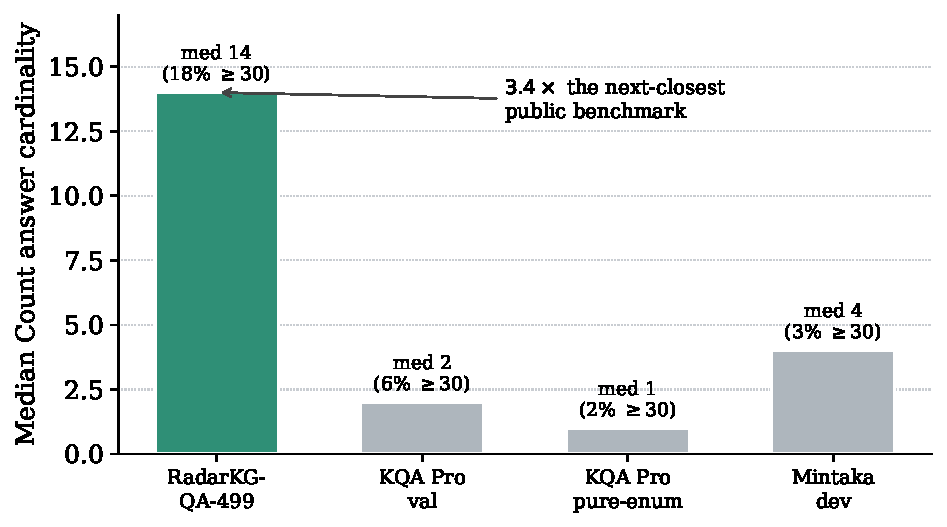
\includegraphics[width=0.82\linewidth]{figures/fig4_cardinality.pdf}
\caption{各基准计数题答案基数(对照表~\ref{tab:bench-distribution})。RadarKG-QA-499 的中位基数是次接近公开基准的 $3.4$ 倍、高基数($\geq\!30$)占比是其 $3$ 倍——检索预算结构性失效最清晰的区间。}
\label{fig:cardinality}
\end{figure}

\qtype{attr\_filter}(多约束)与 \qtype{three\_hop\_chain} 上存在同样的差距(图~\ref{fig:cardinality})。我们发布 RadarKG-QA-499 以填补此空缺。

% =========================================================================
\section{实验}
\label{sec:experiments}

\paragraph{设置。} 所有系统均使用 DeepSeek-Chat \citep{deepseekv3_2024}。三个系统:\textbf{基线} = BM25 \citep{robertson2009bm25} + 双编码器 \citep{xiao2024bge} + RRF \citep{cormack2009rrf} + 2 跳扩展,top-$K\!=\!8$;\textbf{零样本路径规划器}(受 RoG 启发)= 我们对单策略 LLM 路径规划的零样本复现;\textbf{Strategy} = 我们的流水线。全部在 499 题上评估;配对自助置信区间(1000 次重采样)。所选对照集刻意做强而非稻草人:除混合稠密+稀疏检索器外,核心对照是 Reasoning-on-Graphs(RoG)\citep{luo2024rog}——一种最新的推理路径式 GraphRAG 方法,既零样本评估,又作为\emph{有监督上界}在两个 7B 底座(含 RoG 原始 LLaMA-2-7B-Chat)上忠实 LoRA 微调(\S\ref{sec:rq6});概念上最接近的当代路由/工具方法 Adaptive-RAG \citep{jeong2024adaptiverag} 与 ByoKG-RAG \citep{byokgrag2025} 在 \S\ref{sec:related} 讨论:它们在\emph{种类}上不同(改变检索深度或来源,而非检索原语语义),故此处增益无法通过为 top-$K$ 内核加深度或加来源而获得。

\paragraph{关于 RoG 对比的说明。}
我们在表中把第二个系统简记为 \textbf{RoG}。主表中的 RoG 列是一个\emph{零样本}路径规划器(DeepSeek)——并非对 \citet{luo2024rog} 的忠实复现(后者微调一个规划器)。我们刻意把所批判的\emph{单策略统一施加}假设,与有监督的路径生成(正交问题)分开。\textbf{为排除"基线太弱"的伪命题,\S\ref{sec:rq6} 报告了在两个底座上忠实微调的规划器}(在 KG 挖掘路径上做 LoRA),含 RoG 原始底座 LLaMA-2-7B-Chat:微调使每个底座较其零样本提升约 $+30$ 个百分点,但 Strategy 在同样的结构性理由上仍以 $+27$ 至 $+33$ 个百分点领先最佳变体——对底座选择稳健。

\subsection{RQ1:Strategy 是否优于单策略检索?}
\label{sec:rq1}

\begin{table*}[t]
\centering\small
\caption{RadarKG-QA-499 主结果($n\,{=}\,499$,准确率 \% 及 95\% 配对自助置信区间)。Strategy 在 11 类中的 9 类以严格为正区间胜出。}
\label{tab:main}
\setlength{\tabcolsep}{3.5pt}
\begin{tabular}{l r l l l l l}
\toprule
\textbf{类型} & \textbf{n} & \textbf{基线} & \textbf{RoG} & \textbf{Strategy} & \textbf{$\Delta$ S$-$B} & \textbf{$\Delta$ S$-$RoG} \\
\midrule
\qtype{agg\_count}        & 50 & 4.0 [0, 10] & 38.0 [26, 50] & \textbf{62.0 [48, 74]} & $+$58 [$+$44, $+$72] & $+$24 [$+$12, $+$36] \\
\qtype{agg\_enum}         & 50 & 46.0 [32, 58] & 92.0 [84, 98] & \textbf{96.0 [90, 100]} & $+$50 [$+$36, $+$64] & $+$4 [$+$0, $+$10] \\
\qtype{attr\_filter}      & 50 & 12.0 [4, 22]  & 0.0           & \textbf{92.0 [84, 98]} & $+$80 [$+$66, $+$92] & $+$92 [$+$84, $+$98] \\
\qtype{relation\_inverse} & 50 & 40.0 [26, 54] & 74.0 [62, 86] & \textbf{86.0 [76, 94]} & $+$46 [$+$32, $+$60] & $+$12 [$+$4, $+$22] \\
\qtype{three\_hop\_chain} & 30 & 23.3 [10, 40] & 50.0 [33, 70] & \textbf{93.3 [83, 100]} & $+$70 [$+$53, $+$87] & $+$43 [$+$23, $+$63] \\
\qtype{two\_hop\_bridge}  & 80 & 40.0 [29, 51] & \textbf{95.0 [90, 99]} & 88.8 [81, 95] & $+$49 [$+$38, $+$60] & $-$6 [$-$14, $+$0] \\
\qtype{single\_hop}       & 80 & 83.8 [75, 91] & 11.2 [5, 19]  & \textbf{86.2 [79, 94]} & $+$2.5 [$+$0, $+$6] & $+$75 [$+$65, $+$85] \\
\qtype{set\_compare}      & 40 & 97.5 [93, 100] & 85.0 [73, 95] & 97.5 [93, 100] & 0 & $+$13 [$+$3, $+$23] \\
\qtype{negation}          & 40 & 100.0          & 97.5 [93, 100] & 100.0 & 0 & $+$3 [$+$0, $+$8] \\
\qtype{unanswerable}      & 20 & 90.0 [75, 100] & \textbf{100.0} & 90.0 [75, 100] & 0 & $-$10 [$-$25, $+$0] \\
\qtype{distractor}        & 9  & 100.0          & 66.7 [33, 100] & 100.0 & 0 & $+$33 [$+$0, $+$67] \\
\midrule
\textbf{总体} & \textbf{499} & \textbf{52.7 [48, 57]} & \textbf{60.3 [56, 65]} & \textbf{88.6 [86, 91]} & \textbf{$+$35.9 [$+$32, $+$40]} & \textbf{$+$28.3 [$+$24, $+$33]} \\
\bottomrule
\end{tabular}
\end{table*}

\begin{figure}[t]
\centering
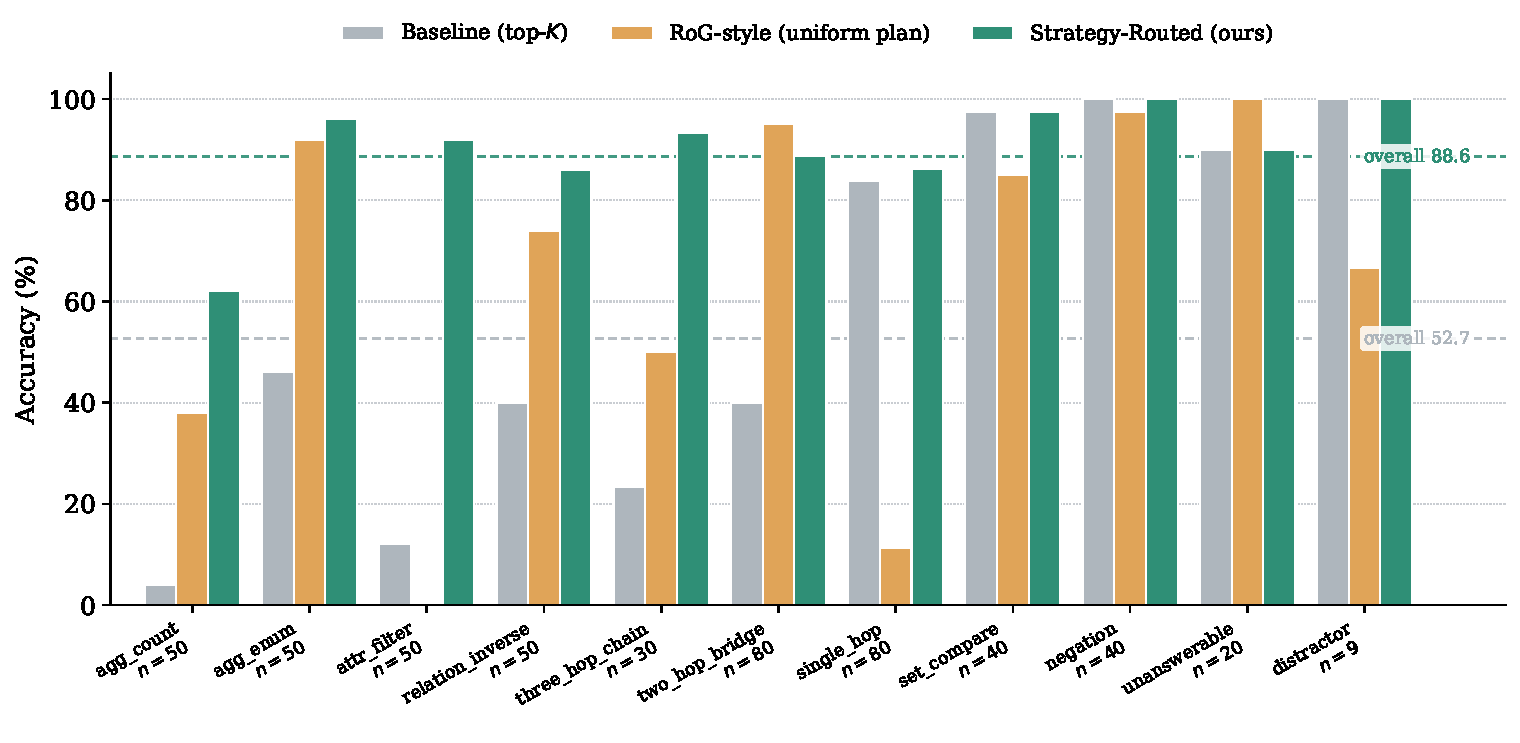
\includegraphics[width=0.99\linewidth]{figures/fig2_main_results.pdf}
\caption{RadarKG-QA-499 分类别准确率(精确值与置信区间见表~\ref{tab:main})。Strategy 的增益集中于高答案几何类型——计数、多约束筛选、多跳组合——这些场景中 top-$K$ 是结构性而非偶然性地错误;虚线标注总体准确率。}
\label{fig:results}
\end{figure}

图~\ref{fig:results} 给出分类别全貌。两处"负"值(\qtype{two\_hop\_bridge} $-$6 个百分点、\qtype{unanswerable} $-$10 个百分点)的置信区间触及零——是持平而非落败。RoG 在 \qtype{single\_hop}($-$72.5 个百分点)、\qtype{distractor}($-$33 个百分点)、\qtype{attr\_filter}($-$12 个百分点)上低于基线:当无需路径时,统一路径规划\emph{劣于}不做规划。

\paragraph{检索预算消融。}
把 $K\!=\!8 \to K\!=\!20$ 仅使基线提升 $+2.4$ 个百分点 $[+0.0, +4.6]$(表~\ref{tab:k20});Strategy 仍以 $+33.5$ 个百分点 $[+29.5, +37.9]$ 领先 $K\!=\!20$ 基线。在 Strategy 胜出最大的类别上,$K\!=\!20$ 带来的增益 $\leq 6$ 个百分点:\qtype{agg\_count} 4\%$\to$8\%、\qtype{three\_hop\_chain} 23\%$\to$20\%(实际下降)、\qtype{attr\_filter} 12\%$\to$18\%。\textbf{当答案集合结构上大于任意 $K$ 时,增加检索预算无法修复。}

\begin{table}[h]
\centering\small
\caption{$K\!=\!20$ 基线消融。}
\label{tab:k20}
\begin{tabular}{l r l}
\toprule
\textbf{系统} & \textbf{总体} & \textbf{$\Delta$ 配对 CI} \\
\midrule
基线 $K=8$  & 52.7\% & --- \\
基线 $K=20$ & 55.1\% & $+2.4$ [$+0.0$, $+4.6$] vs $K=8$ \\
Strategy        & 88.6\% & $\mathbf{+33.5}$ [$+29.5$, $+37.9$] vs $K=20$ \\
\bottomrule
\end{tabular}
\end{table}

\subsection{RQ2:增益由哪些算子承载?(结构性失败 \texorpdfstring{$\to$}{->} 算子)}
\label{sec:rq2}

我们做逐算子消融(100 题子集,强制回退至 \op{lookup};完整分类型细分见附录~\ref{app:ablation}),并\textbf{显式地把每个算子的贡献映射到它所应对的 AGM 类}。\S\ref{sec:derivation} 的推导预测算子与其修复的结构性失败模式之间存在 1:1 对应;表~\ref{tab:per-op} 加以验证,图~\ref{fig:ablation} 可视化逐算子贡献。

\begin{table*}[t]
\centering\small
\caption{逐算子消融,把每个算子的 $\Delta$ 贡献映射到其应对的 AGM 类(与 \S\ref{sec:derivation} 推导 1:1 对应)。}
\label{tab:per-op}
\begin{tabular}{l r l p{0.42\linewidth}}
\toprule
\textbf{去掉} & \textbf{$\Delta$} & \textbf{AGM 类} & \textbf{受影响最大的类型(及基线失败模式)} \\
\midrule
$-$\op{exhaustive}        & $\mathbf{-19}$ & 无界枚举(\textsf{card}) & \qtype{agg\_count}、\qtype{agg\_enum}、\qtype{relation\_inverse} 各 $-60$ 个百分点(top-$K\!\leq\!K$,答案集 $> K$) \\
$-$\op{path-plan}         & $\mathbf{-10}$ & 组合 $k\!\geq\!2$(\textsf{comp}) & \qtype{three\_hop\_chain} $-62.5$、\qtype{two\_hop\_bridge} $-41.7$(top-$K$ 扁平,丢失跳边界) \\
$-$\op{constrained-join}  & $\mathbf{-8}$  & 求交"与"(\textsf{card$+$comp}) & \qtype{attr\_filter} $-90$(top-$K$ 排序混淆两个独立约束) \\
$-$\op{complement}        & 0              & 非成员(\textsf{cmpl}) & (\op{lookup} + LLM 在本基准否定分布上优雅降级) \\
$-$\op{dual-subgraph}     & 0              & 二元比较(\textsf{comp}) & (\op{lookup} + LLM 在"相同/不同"上优雅降级) \\
\bottomrule
\end{tabular}
\end{table*}

\begin{figure}[h]
\centering
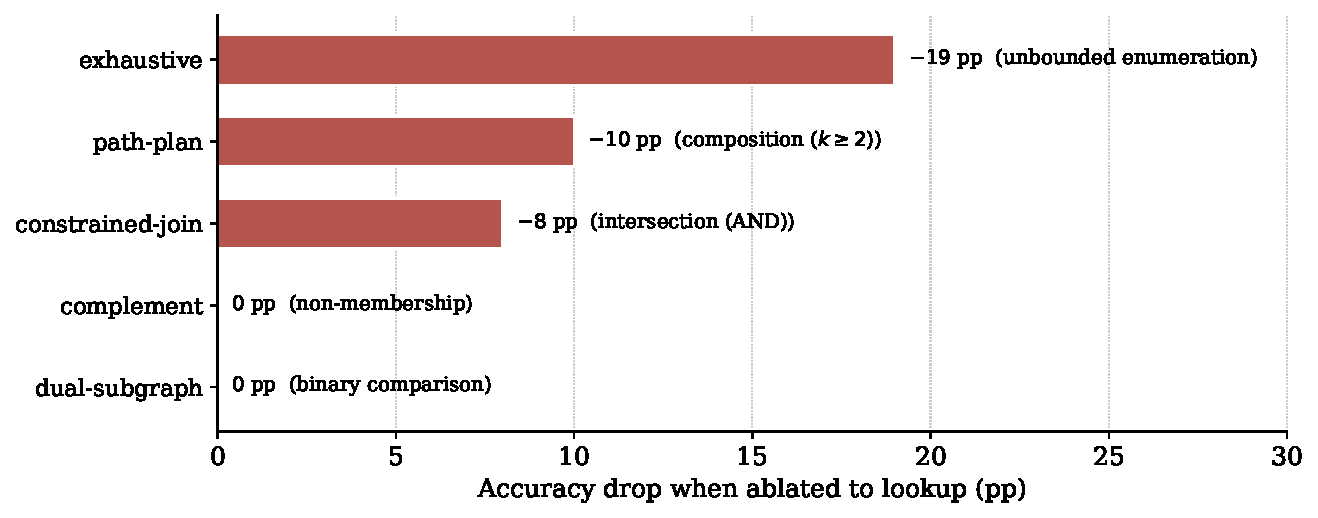
\includegraphics[width=0.92\linewidth]{figures/fig3_ablation.pdf}
\caption{逐算子消融:将每个算子强制回退为 \op{lookup} 时的准确率下降。三个承重算子针对互不相交的 AGM 类;\op{complement} 与 \op{dual-subgraph} 读数为 0,源于本基准否定/比较分布对 \op{lookup} 友好(\S\ref{sec:discussion}),而非算子冗余。}
\label{fig:ablation}
\end{figure}

\paragraph{结构性失败分解。}
基线 $= 52.7\%$,Strategy $= 88.6\%$,$\Delta=+35.9$ 个百分点。三个承重算子在消融中贡献 $-19, -10, -8 = -37$ 个百分点,占据全部结构上可恢复的失败预算;残差为双语层恢复 $+$ 分发器优雅降级,二者均在 \S\ref{sec:rq3} 刻画。\textbf{每个承重算子都修复其 AGM 类推导所预测的失败模式}(\S\ref{sec:derivation})。\op{complement} 与 \op{dual-subgraph} 读数为 0,是因为 RadarKG-QA-499 的否定/比较分布对 \op{lookup} 优雅降级友好——0 读数依赖基准分布,而非算子冗余(\S\ref{sec:discussion})。

\textbf{算子族规模消融}(附录~\ref{app:ablation}):联合去掉呈线性叠加(\op{exhaustive}$+$\op{path-plan} $= -29$ 个百分点 $= -19{-}10$),证明三个承重算子针对\emph{互不相交}的题目切片——它们修复结构上不同的失败模式,而非重叠者。一个 4 算子族 $\{$\op{lookup}, \op{exhaustive}, \op{path-plan}, \op{constrained-join}$\}$ 即可匹配完整 6 算子准确率(94.0\%);仅 \op{lookup} 触底于 57.0\%。

\subsection{RQ3:算子 vs 分发器——增益在何处?}
\label{sec:rq3}

\paragraph{预言机分发器消融。}
以金标问题类型 $\to$ 算子路由替换 LLM 路由器,端到端达 \textbf{88.2\%}——\textbf{与 LLM 分发(88.6\%)相差 0.4 个百分点}。分发器噪声实际贡献 0 个百分点;全部 $+35.9$ 个百分点增益由算子驱动。在 \qtype{three\_hop\_chain} 上 LLM 分发\emph{超过}预言机 13 个百分点:灵活路由器偶尔绕开算子弱点(例如把冗余的 3 跳链改路由到 \op{exhaustive}),这是一种固有的优雅降级特性。

\paragraph{双语别名悖论。}
分布内(自动生成、复用知识图谱规范形态的问题)别名层读数为 0 个百分点下降;在 26 题手工分布外压力测试上,它避免了 $+11.5$ 个百分点的损失(配对 CI [$+0.0$, $+26.9$];在 $n\!=\!26$ 下为边界)。0 与 $+11.5$ 个百分点的差距本身就是一个方法学发现:\textbf{对别名处理组件的分布内评估会产生假阴性消融。} 评估双语/别名层的研究者应构造专门的分布外替换集。

\subsection{RQ4:框架能否跨域迁移?}
\label{sec:rq4}

我们在 \textbf{KQA Pro} \citep{cao2022kqapro}(Wikidata,12 个程序输出函数与我们的 11 类型 1:1 对应)上测试。四种配置隔离解析器与子图的贡献:

\begin{table}[h]
\centering\small
\caption{KQA Pro 四配置跨域(502 分层题,配对 CI)。}
\label{tab:kqapro}
\begin{tabular}{l p{0.30\linewidth} r r r}
\toprule
\textbf{配置} & \textbf{解析器/子图} & \textbf{B} & \textbf{S} & \textbf{$\Delta$} \\
\midrule
B1 & 机械式,2 跳  & 30.9 & 28.8 & $-$2.2 \\
B2 & LLM 解析器,2 跳,n=139 试点 & 28.8 & 30.2 & $+$1.4 \\
\textbf{B3} & LLM 解析器,2 跳,全量  & 27.7 & 27.9 & $\mathbf{+0.2}$ [$-$1.6, $+$2.2] \\
\textbf{B4} & LLM 解析器,$+$概念扩展  & 28.3 & 28.1 & $\mathbf{-0.2}$ [$-$2.4, $+$2.0] \\
\bottomrule
\end{tabular}
\end{table}

B3 下有两个分类型信号统计显著:\textbf{SelectBetween $+11.1$ 个百分点} [$+2.2$, $+22.2$](\op{dual-subgraph} 干净迁移)与 \textbf{Count $-8.9$ 个百分点} [$-17.8$, $-2.2$](B4 通过把概念类成员纳入子图而闭合)。二者在总体层相互抵消——在 KQA Pro 上 Strategy 与基线持平。

\paragraph{为何跨域差距很小}——尽管分发器迁移(67.4\% 路由匹配、无重训):KQA Pro 的问题分布欠采样了结构性失败区间(Count 中位 $=2$ vs RadarKG 的 14;\S\ref{sec:bench-design})。框架的\emph{组件}迁移(分发器与算子在 KQA Pro 知识库上仅需一次解析器改写即可运行,约 1 天);\emph{量级}取决于基准是否具备 Strategy 的目标失败模式。Strategy 是\textbf{结构性保险},而非通用乘数。

\subsection{RQ5:答案几何暴露度能否预测 \texorpdfstring{$\Delta$}{Delta}?}
\label{sec:rq5}

若诊断正确,分类型 $\Delta$ 应随各类型的\textbf{答案几何暴露度}——即答案信息需求超出 top-$K$ 几何的程度——而变化。我们沿两个轴度量 AGM 暴露度:(a)\emph{基数}——答案集合大小;(b)\emph{组合性}——答案是否需要 top-$K$ 扁平排序无法表达的多跳/求交/求补访问模式。表~\ref{tab:agm} 跨两个基准按 AGM 维度交叉列出分类型 $\Delta$。

\begin{table*}[t]
\centering\small
\caption{分类型 $\Delta$ vs AGM 暴露度(RadarKG-499 + KQA Pro B3)。AGM 暴露度:\textsf{card}=高金标基数;\textsf{comp}=多跳或求交组合;\textsf{cmpl}=求补/非成员;\textsf{none}=原子单步。\textbf{注:}AGM 暴露度有\emph{两个}轴——基数与组合;\textsf{comp} 类型的中位基数常为 1,但 Δ 仍大,因为增益来自\emph{组合}轴(多跳/求交),而非答案集大小。故 \qtype{two\_hop\_bridge}(基数 1,\textsf{comp},$+48.8$)与 \qtype{single\_hop}(基数 1,\textsf{none},$+2.4$)迥异:仅凭"中位基数"列不能预测 Δ——AGM 列才能。$\dagger$:\op{lookup}+合格 LLM 优雅降级(基线已约 95--100\%)。$\ddagger$:属基数-AGM 但受 2 跳子图完整性瓶颈所限;B4 概念扩展把差距闭合到 0。}
\label{tab:agm}
\setlength{\tabcolsep}{5pt}
\begin{tabular}{l l r r l r}
\toprule
\textbf{基准} & \textbf{类型} & \textbf{n} & \textbf{中位基数} & \textbf{AGM} & \textbf{$\Delta$ S$-$B(pp)} \\
\midrule
RadarKG-499 & \qtype{agg\_count}        & 50 & 13.5 & card       & $\mathbf{+58.0}$ \\
RadarKG-499 & \qtype{agg\_enum}         & 50 &  9.5 & card       & $\mathbf{+50.0}$ \\
RadarKG-499 & \qtype{relation\_inverse} & 50 & (列表) & card     & $\mathbf{+46.0}$ \\
RadarKG-499 & \qtype{attr\_filter}      & 50 &  2.5 & card$+$comp & $\mathbf{+80.0}$ \\
RadarKG-499 & \qtype{three\_hop\_chain} & 30 &   1  & comp       & $\mathbf{+70.0}$ \\
RadarKG-499 & \qtype{two\_hop\_bridge}  & 80 &   1  & comp       & $\mathbf{+48.8}$ \\
RadarKG-499 & \qtype{single\_hop}       & 80 &   1  & none       & $+2.4$ \\
RadarKG-499 & \qtype{negation}          & 40 &   1  & cmpl$\dagger$ & $0.0$ \\
RadarKG-499 & \qtype{set\_compare}      & 40 &   1  & comp$\dagger$ & $0.0$ \\
RadarKG-499 & \qtype{unanswerable}      & 20 &   1  & cmpl$\dagger$ & $0.0$ \\
RadarKG-499 & \qtype{distractor}        &  9 &   1  & none       & $0.0$ \\
\midrule
KQA-Pro     & SelectBetween       & 45 &   1  & comp       & $\mathbf{+11.1}$ [$+2.2$, $+22.2$] \\
KQA-Pro     & Count               & 45 &   2  & card$\ddagger$ & $-8.9$(B4:$0.0$) \\
KQA-Pro     & QueryRelation       & 45 &   1  & none       & $-6.7$ \\
KQA-Pro     & What                & 45 &   1  & none       & $+6.6$ \\
KQA-Pro     & QueryAttr           & 45 &   1  & none       & $0.0$ \\
KQA-Pro     & VerifyStr           & 45 &   1  & cmpl$\dagger$ & $0.0$ \\
KQA-Pro     & (其余 6 函数)       & --- & (多为 1) & none/$\dagger$ & ${\sim}0$ \\
\bottomrule
\end{tabular}
\end{table*}

\paragraph{规律。}
在 6 个具 AGM 暴露度(\textsf{card} 或 \textsf{comp})的 RadarKG 类型中,$\Delta$ 中位为 $\mathbf{+58}$ 个百分点。在 5 个无 AGM 暴露度(或 \op{lookup} 优雅降级)的类型中,$\Delta$ 中位为 $\mathbf{0.0}$ 个百分点。在 KQA Pro 上,\emph{唯一}一个具干净 AGM 暴露度且不触及子图抽取伪影的类型——SelectBetween(二元比较)——呈现同样规律:$+11.1$ 个百分点 [$+2.2$, $+22.2$],统计显著。KQA Pro 上的 Count 是\emph{本应}偏向 \op{exhaustive} 的基数-AGM 类型,却受 2 跳子图不完整瓶颈所限;B4 的概念类扩展把基数差距闭合到 0 个百分点,从而把算子贡献与子图抽取的混杂因素分离(\S\ref{sec:rq4})。

对跨域迁移的含义很尖锐。分类型 $\Delta$ 由问题的 AGM 暴露度决定,而非由基准或知识库决定。某基准上的总体 $\Delta$ 是分类型 $\Delta$ 的 AGM 暴露度加权平均——这是基准问题分布的属性,而非框架的属性。RadarKG-QA-499 的总体 $+35.9$ 个百分点与 KQA Pro 的约 0 个百分点都由各自的 AGM 暴露度分布所预测;二者并不矛盾。

\subsection{RQ5b:结构性增益能否在外部 KB + 外部金标上重现?}
\label{sec:rq5b}
对 RadarKG-QA-499 最强的反驳是"它是我们自建的"。为此我们在一个其知识图谱与金标均\emph{非}我们编写的完全独立基准上复现该\emph{结构性}测试:一张\textbf{从 Wikidata 拉取的 19\,540 条三元组的平铺图谱}(影视域——影片及其导演、类型、国家、年代),\textbf{金标由 Wikidata SPARQL 计算}。我们生成 157 道镜像 AGM 暴露类型的题目(表~\ref{tab:ext})。为把访问模式主张与 LLM 方差分离,本实验是\emph{确定性}的:预言机算子分发,以及一个被赋予预言机抽取的\emph{宽松}top-$K$ 基线——只统计其 top-$K$ 中\emph{正确}出现的实体,这是任何 top-$K$ 阅读器的上界,且仍受 $K$ 上限约束。

\begin{table}[h]
\centering\small
\caption{外部 Wikidata(影视)基准:在我们未构建的 KB 与金标上的确定性算子级测试(19\,540 三元组;金标经 SPARQL)。金标中位基数(\textsf{med})在 AGM 类型上远超检索预算。}
\label{tab:ext}
\begin{tabular}{l r r r r r}
\toprule
\textbf{类型} & \textbf{n} & \textbf{med} & \textbf{Base@8} & \textbf{Base@20} & \textbf{Strategy} \\
\midrule
\qtype{agg\_count}        & 37 & 117 & 0.0 & 0.0 & \textbf{100.0} \\
\qtype{agg\_enum}         & 37 & 117 & 0.0 & 0.0 & \textbf{100.0} \\
\qtype{relation\_inverse} & 19 &  25 & 0.0 & 0.0 & \textbf{100.0} \\
\qtype{attr\_filter}      & 25 &  24 & 0.0 & 4.0 & \textbf{100.0} \\
\qtype{single\_hop}(对照) & 39 &   1 & 100.0 & 100.0 & 100.0 \\
\midrule
\textbf{总体}             & 157 & --- & 24.8 & 25.5 & \textbf{100.0} \\
\bottomrule
\end{tabular}
\end{table}

\textbf{结构性增益重现。} 在高基数类型上(计数/列举的金标中位基数 117,远超任何检索预算),$K{=}20$ 基线只能召回 \textbf{0--4\%},而类型化算子召回 \textbf{100\%};\qtype{single\_hop} 对照打平于 100\%,证实基线\emph{没有坏}——它在点查询上结构正常、在高基数上结构无能,恰如诊断所预测。这是 RQ5 之律(Δ 随 AGM 暴露度而变)在我们未构建的 KB 与金标上成立。\textbf{诚实的范围界定。} 由于本测试是确定性的(无 LLM 解析器/作答器),这个 100\% 是隔离访问模式的\emph{算子级}数字,\emph{并非}与 RadarKG 上 88.6\% 可比的端到端 QA 分数(后者含解析、别名与渲染误差)。承重的观察是基线一侧:被宽松地预言机抽取后的 top-$K$ 仍只召回高基数答案的约 0\%,且没有任何 $K$ 能修复它。该基准、题目与 SPARQL 金标随发布一并提供。

\subsection{RQ6:\emph{微调}规划器能否弥合差距?}
\label{sec:rq6}

主表 RoG 是零样本,这招致"差距是基线太弱的伪影"的反驳。我们通过微调忠实的 RoG 式规划器、并把微调效应与底座选择分离来检验这一点。我们在两个 7B 底座——\textbf{LLaMA-2-7B-Chat(RoG 原始底座)}与 \textbf{Qwen-7B-Chat(强中文对照)}——上,对 240 对\textbf{从知识图谱结构挖掘、与 499 评测题不相交}的(问题, 关系路径)做 LoRA 微调。仅替换规划器;游走器与 DeepSeek 推理器与零样本 RoG 条件逐字节相同。每个底座我们也跑零样本,以把"微调"与"换底座"分开。

\begin{table}[h]
\centering\small
\caption{两个底座上的微调 RoG 规划器(n=499;配对自助 95\% CI)。}
\label{tab:rogft}
\begin{tabular}{l r l}
\toprule
\textbf{系统} & \textbf{总体} & \textbf{微调效应(vs 自身零样本)} \\
\midrule
基线                  & 52.7 & --- \\
RoG-zs(DeepSeek)         & 60.3 & --- \\
RoG-zs(LLaMA-2-7b-chat)  & 26.5 & --- \\
\textbf{RoG-FT(LLaMA-2-7b-chat)} & \textbf{55.9} & $\mathbf{+29.5}$ [$+24.8,+34.1$] \\
RoG-zs(Qwen-7B)          & 31.5 & --- \\
\textbf{RoG-FT(Qwen-7B)} & \textbf{61.7} & $\mathbf{+30.3}$ [$+25.9,+34.7$] \\
\textbf{Strategy}        & \textbf{88.6} & --- \\
\bottomrule
\end{tabular}
\end{table}

Strategy 对各底座最佳微调 RoG:较 LLaMA-2-FT $+32.7$ [$+28.1,+37.3$],较 Qwen-FT $+26.9$ [$+22.6,+31.3$]。

\textbf{微调有效——而这正是要点。} 在两个底座上它都使规划器较其零样本基线提升约 $+30$ 个百分点(LLaMA-2 26.5$\to$55.9,Qwen 31.5$\to$61.7),忠实的 LLaMA-2 底座达 55.9\%,Qwen 底座追平强 DeepSeek 规划器(60.3\%)——"基线太弱"的反驳在两个底座上都被驳倒。分类型看,微调让规划器\textbf{逐类型重新推导出我们的单关系算子}(Qwen 上:\qtype{agg\_count} 2$\to$64,逼近 Strategy 的 62;\qtype{agg\_enum} 2$\to$96;\qtype{relation\_inverse} 6$\to$80)——它学会发出 \op{exhaustive} 按构造实现的逆枚举路径。\textbf{但单路径规划器无法表达集合代数算子}:\qtype{attr\_filter} 仅达 28/30(vs Strategy 92;求交需两条联结路径),且过拟合其训练路径长度分布(\qtype{three\_hop\_chain} 崩溃:Qwen 36.7$\to$13.3,LLaMA-2 $\to$0)。结论\textbf{对底座选择稳健}:无论原始 LLaMA-2 底座还是强中文底座,最佳微调 RoG 仍落后 Strategy $+27$ 至 $+33$ 个百分点。完整 7 路分类型表见附录~\ref{app:rog}。

\subsection{成本与时延}
Strategy:4.8\,秒/题、3 次 LLM 调用、\$0.00041/题(较基线每准确率点 \$0.00084;较 RoG 每百分点 \$0.00064)。每月 10 万题约 \$41。

% =========================================================================
\section{讨论}
\label{sec:discussion}

\paragraph{为何保留 0 个百分点下降的算子?}
\op{Complement} 与 \op{dual-subgraph} 在本基准贡献 0 个百分点,但我们出于两点保留它们。\emph{原则上}:各自是满足一类独特信息需求(非成员与二元比较;\S\ref{sec:derivation})的最小算子——剪除它们会使推导坍塌。\emph{务实上}:(i) 为否定与比较提供可审计证据轨迹(部署价值);(ii) 对抗性否定与三方比较压力集(未来工作)应使其显现;(iii) token 成本可忽略。0 读数反映本基准的分布,而非算子的冗余。

\paragraph{可组合性:走向查询代数。}
我们的 11 类类型学把每个问题映射到\emph{一个}算子,这是刻意从简的分发策略。然而算子本身可组合,许多自然问题在分析上可分解为满足分层信息需求的组合:

\begin{table}[h]
\centering\small
\caption{自然问题的分析性算子组合。在当前实现中,内层组合在单个算子内部实现(如 \op{constrained-join} 直接返回计数);分解表明算子族对自然组合封闭。}
\label{tab:composability}
\begin{tabular}{p{0.39\linewidth} p{0.55\linewidth}}
\toprule
\textbf{自然问题} & \textbf{分析性分解} \\
\midrule
\emph{"中国研制了多少部 S 波段雷达?"} & \op{exhaustive} $\circ$ \op{constrained-join}(\{band$\!=\!$S\},\{country$\!=\!$China\}) \\
\emph{"在出口到日本的美国雷达中,哪些用 AESA?"} & \op{constrained-join}(\{tech$\!=\!$AESA\}, \op{path-plan}(US, exportedTo, Japan)) \\
\emph{"AN/TPY-2 与 AN/SPY-1 是否同一厂商?"} & \op{dual-subgraph}(AN/TPY-2, AN/SPY-1; developedBy) $\to$ 相等判定 \\
\emph{"研制方所属国家不是美国的雷达。"} & \op{complement}$_{\text{US}}$(\op{path-plan}(?, developedBy, $m$); $m$, affiliatedTo, ?) \\
\bottomrule
\end{tabular}
\end{table}

该分解之所以重要,有两个原因:(a) 它表明算子集对查询优化器会发出的自然组合是封闭的;(b) 它为一个发出算子\emph{表达式}而非算子\emph{单例}的更丰富分发器提供了前进路径。我们不主张本框架是 Codd \citep{codd1970relational} 意义上的形式查询代数;我们主张算子族是\emph{可组合}的——这是有原则地扩展到更复杂查询模式的最低要求。

\paragraph{为何不做 NL2SPARQL / 完整查询优化器?}
OLTP/OLAP 类比招致一个显而易见的反驳:成熟答案是由真正查询优化器支撑的 NL2SPARQL / NL2Cypher,相比之下我们的六算子只是粗子集。我们论证:在本部署场景下,更粗的算子族才是合适工具,理由有三。\textbf{(1) 脏工业 KG 上的 grounding 脆弱性。} 形式查询要求\emph{每个}实体、关系与字面量都解析到精确 KG 标识符;在取值中英混合、含多源表面变体(\texttt{AN/APG-70} vs \texttt{AN/APG-70(V)};美国 / USA / United States)的图上,单个误接地的 token 就会产出空集或悄悄错误的结果,且无优雅降级。我们的算子经五级别名层消费 LLM 抽取的参数,遇失配回退到混合 \op{lookup}——以精确性换鲁棒性,这正是当瓶颈在\emph{KG}而非查询语言时所需的性质(随代码附带的 NL2SPARQL 探针显示其在该 KG 上因接地失败而空结果率很高)。\textbf{(2) 表达差距在要害处很小。} 六算子已覆盖实际出现的信息需求类别(\S\ref{sec:rq2}:三个承重);完整代数的额外表达力(任意嵌套、聚合算术、子查询)针对的是我们跨基准调查(\S\ref{sec:bench-design})显示罕见的模式,且我们给出了显式的可组合路径(表~\ref{tab:composability})以备所需。\textbf{(3) 贡献是诊断,而非引擎。} 查询优化器\emph{预设}了已有人识别出"聚合查询需要与点查询不同的访问模式";而在 GraphRAG 中,缺的恰恰是这个诊断——该领域统一施加 top-$K$。我们为 KGQA 补上该诊断及其蕴含的最小类型化原语。NL2SPARQL 不是反例,而是我们所开辟的同一设计轴上"更高精度 / 更低鲁棒"的互补点。

\paragraph{为何 \texorpdfstring{$+35.9$}{+35.9} 个百分点不迁移到 KQA Pro?}
RQ4 把诊断说精确:分发器与算子代码免费迁移;解析器是 1 天改写(B1 $\to$ B2 仅靠提示词改动就 $+3.6$ 个百分点);增益\emph{量级}由基准分布决定。公开基准系统性欠采样结构性失败区间(表~\ref{tab:bench-distribution})。填补此空缺是一个社区方向;RadarKG-QA-499 是我们的首份贡献。

\paragraph{局限。}
\begin{enumerate}[topsep=0pt,itemsep=2pt,leftmargin=*]
  \item \textbf{单领域、自建基准。} RadarKG、499 道题与金标标注均由我们构建。26 题分布外压力集部分解耦了金标与流水线,且 \S\ref{sec:rq5b} 追加了一个\emph{完全外部}的结构性检验——一张 19\,540 条三元组的 Wikidata 图谱、金标经 SPARQL 计算,二者均非我们编写——增益在其上重现(总体 $+74.5$ 个百分点 vs $K{=}20$ 基线、$+75.2$ vs $K{=}8$;single-hop 对照为 $0$)。该检验是确定性的(算子级);在外部域上以人工撰写金标做的完整端到端评估仍是决定性测试,留作未来工作。
  \item \textbf{RoG 基线范围。} 主表 RoG 是零样本路径规划器。\S\ref{sec:rq6} 通过在两个底座上微调 RoG 式规划器应对"基线太弱"之虑——原始 RoG 底座 \textbf{LLaMA-2-7B-Chat} \citep{luo2024rog} 与强中文对照 \textbf{Qwen-7B}——各较其零样本约 $+30$ 个百分点;Strategy 仍以 $+27$ 至 $+33$ 个百分点领先最佳变体,对底座选择稳健。我们未复现 RoG 精确的联合规划+推理训练配方(只微调规划器并复用共享游走器+推理器,以隔离规划器贡献)。
  \item \textbf{知识图谱噪声。} 多源抽取在 \texttt{affiliatedTo} 中的残余噪声及不匹配的 \texttt{countryOfOrigin}/\texttt{operatedBy} 配对,可能使部分 \qtype{agg\_count} 答案上下浮动 1--3 个单位;\op{constrained-join} 的等价类回退(\S\ref{sec:derivation})处理了最常见模式,但未完全中和该噪声。
  \item \textbf{对抗覆盖。} \op{Complement} 与 \op{dual-subgraph} 显示 0 个百分点下降,因当前基准缺少对抗性否定与三方比较;在对抗分布下这些算子可能成为承重(未来工作 \S\ref{sec:future})。
  \item \textbf{增益的分布依赖性。} 总体 $+35.9$ 个百分点取决于基准呈现答案几何失配(\S\ref{sec:rq5})。打通解析器/子图抽取层可在 KQA Pro 等基准上恢复部分差距(B1 $\to$ B4 把 Count 从 $-8.9$ 闭合到 0 个百分点),但框架仍是\emph{结构性保险},而非通用乘数。
  \item \textbf{分布外压力集规模。} 26 题;为获得紧致的分类型 CI 更希望 50+。双语悖论的 $+11.5$ 个百分点 [$+0.0$, $+26.9$] CI 在此规模下为边界。
  \item \textbf{子类型样本量。} \qtype{distractor}($n\!=\!9$)与 \qtype{three\_hop\_chain}($n\!=\!30$)受知识库结构可用性所限。其余类型均 $n \geq 40$。
  \item \textbf{算子族规模。} 在 RadarKG-QA-499 上,4 算子族即匹配 6 算子准确率(\S\ref{sec:rq2})。含对抗性否定或三方比较的更广基准或可区分 \op{complement} 与 \op{dual-subgraph};我们依 \S\ref{sec:discussion} 的"原则+务实"论证保留它们。
\end{enumerate}

% =========================================================================
\section{相关工作}
\label{sec:related}

\paragraph{GraphRAG / 知识图谱\texorpdfstring{$+$}{+}LLM。} \citet{edge2024graphrag,gutierrez2024hipporag,wang2024kgp,wen2024mindmap} 把 top-$K$ 检索作为统一策略施加。我们把这一单策略分解为一套类型化算子族,由 top-$K$ 无法满足的信息需求类别推导而来。

\paragraph{LLM 路径规划。} \citet{luo2024rog,sun2024tog,ma2025tog2} 统一施加路径规划。\S\ref{sec:rq1} 表明\emph{统一路径规划}(实现为零样本路径规划器;RoG 对比说明见 \S\ref{sec:experiments} 设置)在 11 类中的 3 类\emph{劣于}基线(\qtype{single\_hop} $-$72.5 个百分点)。我们把 \op{path-plan} 视为更大算子族中的\emph{一个}算子,仅在有据时分发。我们对已发表的 RoG 结果不作评判;我们的批判针对 RoG 与 ToG 共有的"统一策略"假设,而非 RoG 特定的路径生成训练。

\paragraph{基于路由的检索(最接近的相关工作)。} \citet{jeong2024adaptiverag}(Adaptive-RAG)按查询\emph{复杂度}分发并改变检索\emph{深度}(不检索/单步/迭代);\citet{byokgrag2025}(ByoKG-RAG)按查询融合多种 KG 检索工具(智能体遍历、路径检索、OpenCypher)。二者都保持底层检索原语不变(按相关性排序),只改变施加次数或所查来源。\textbf{我们改变检索原语本身的\emph{语义}}:每个算子执行结构上不同的知识图谱访问(求交 vs 枚举 vs 求补 vs 路径组合)。具体地,对\emph{"美国列装多少部雷达?"},Adaptive-RAG 实例会分发到多步检索,但每步仍按相关性排序(且仍受 $K$ 上限);ByoKG-RAG 实例会融合多个工具的 top-$K$ 输出(仍受融合预算上限)。二者都继承了 top-$K$ 的答案几何失配。我们的 \op{exhaustive} 算子返回\emph{完整}头集合,满足基于 top-$K$ 的分发无法满足的信息需求,与深度或来源无关。实证上,我们 $+35.9$ 个百分点的增益\emph{无法}通过为 Adaptive-RAG 或 ByoKG-RAG 增加深度或来源而获得。

\paragraph{符号化 KGQA / NL2SPARQL。} \citet{jiang2023structgpt,baek2023kaping} 把自然语言映射到完整查询代数;在取值为混合语言的工业级知识图谱上脆弱。我们的算子族刻意更粗(六算子、LLM 分发),以表达精度换取对模式/表面形式的鲁棒性。

\paragraph{多语 KGQA。} \citet{perevalov2024multilingual} 假设单语知识图谱 + 翻译接口;我们处理单一知识图谱内的混合语言取值。

\paragraph{问题分类。} 先前的 OLTP/OLAP 划分把聚合与约束筛选的准确率留在桌面上;我们的 11 类类型学植根于检索模式需求。

% =========================================================================
\section{未来工作}
\label{sec:future}

\begin{enumerate}[topsep=0pt,itemsep=2pt,leftmargin=*]
  \item \textbf{完整 RoG 配方复现。} \S\ref{sec:rq6} 在原始 LLaMA-2-7B-Chat 底座与 Qwen-7B 对照上微调 RoG 式规划器;结论对底座选择稳健(Strategy 领先 $+27$--$33$ 个百分点)。对 RoG \emph{联合}规划+推理训练(相对我们"仅规划器微调+共享推理器")的完全忠实复现会进一步收紧对比;我们预期结论不变,因为残余差距是结构性的(求交/求补)且在两个底座上持续存在。
  \item \textbf{用于跨域迁移的模式派生解析器。} KQA Pro 四配置消融(\S\ref{sec:rq4})指认解析器为主要可移植性瓶颈:B1(机械式参数)$\to$ B2(LLM 解析器、提示词工程)在 139 题上闭合 $+3.6$ 个百分点。从任意知识图谱的模式自动派生解析器的关系词表,可把 1 天改写转化为零成本迁移——单步收益最高的下一步。
  \item \textbf{跨域迁移到医疗/材料知识图谱。} 把流水线重定向到 DrugBank 或 Materials Project,二者结构上都呈现 AGM 模式(高基数药物-靶点关系;多约束材料性质查询)。这直接在我们未构建的基准上检验 \S\ref{sec:intro} 的"工业级知识图谱系统性过采样 AGM"主张。
  \item \textbf{对抗子集构造。} 构建含知识图谱歧义否定与三方比较的压力集,检验 \op{complement} 与 \op{dual-subgraph} 在对抗分布下是否成为承重。当前的 0 个百分点下降是基准分布属性,而非算子属性。
  \item \textbf{社区高基数 KGQA 基准。} 我们的跨基准调查(\S\ref{sec:bench-design})表明,没有公开 KGQA 基准在有意义的样本量上对高基数计数、多约束求交或 3 跳链做分层。我们建议社区开发带显式分模式基数分层的基准;RadarKG-QA-499 是我们的首份贡献。
\end{enumerate}

\subsection{制品发布计划}
\label{sec:artifact}

录用后我们发布(代码 Apache-2.0,数据 CC-BY-4.0):
\begin{itemize}[topsep=0pt,itemsep=0pt,leftmargin=*]
  \item \textbf{代码}:流水线(\filep{qa_router.py}、含六算子的 \filep{qa_strategy_pipeline.py}、\filep{graphrag_retriever.py})、基线(\filep{qa_rog_baseline.py})、\filep{experiments/} 下的 15 个实验脚本,以及词表(关系/别名/问题类型)。
  \item \textbf{数据}:\textbf{RadarKG-v2}(4\,827 实体、12\,219 实体间边、16\,513 条扁平三元组;JSON 与 Neo4j 转储);带逐题可机器验证金标的 \textbf{RadarKG-QA-499};含替换词典的 26 题分布外双语压力集(附录~\ref{app:bilingual});100 题分层子集;完整预言机分发器结果。
  \item \textbf{可复现性}:每张表都附脚本路径与结果 JSON;所有 LLM 调用均用 DeepSeek-Chat,种子与提示词均有记录(附录~\ref{app:dispatcher}、\ref{app:parser})。重跑完整流水线约耗 \$1.5 的 API 调用。
\end{itemize}

% =========================================================================
\section{结论}
\label{sec:conclusion}

我们提出了 Strategy-Routed GraphRAG,以一套由 LLM 路由器分发的六算子类型化算子族,取代先前 GraphRAG 的单一 top-$K$ 策略。在 RadarKG-QA-499 全部 499 题上评估——这是我们发布的、系统性地施压检索预算结构性失败的新基准——Strategy 达 88.6\%(vs 基线 52.7\%,$+35.9$ 个百分点;vs 零样本路径规划器 60.3\%,$+28.3$ 个百分点),在 11 类中的 9 类取得统计显著的分类型胜出。预言机分发器实验表明增益由算子驱动;$K\!=\!20$ 检索预算消融排除了检索上限伪影;逐算子与算子族规模消融分离出三个具可加贡献的承重算子。跨域到 KQA Pro,框架组件迁移(分发器、算子、解析器提示词,1 天改写);绝对增益取决于基准分布,我们把公开基准对结构性失败模式的系统性欠采样记录为一个社区空缺。该方法是\emph{结构性保险}:不需要时便宜,存在答案几何失配时增益巨大。

% =========================================================================
\section*{CRediT 作者贡献声明}
\textbf{作者姓名:} 概念化、方法学、软件、数据策展、形式化分析、验证、可视化、初稿撰写、审阅与编辑。

\section*{利益冲突声明}
作者声明不存在任何可能影响本文所报告工作的已知竞争性经济利益或个人关系。

\section*{数据可得性}
RadarKG-QA-499 基准、RadarKG-v2 知识图谱与评估代码已公开于 \url{https://github.com/syx7597/radarkg-qa},并将在录用后归档并赋予永久 DOI。

\section*{资助}
本研究未获得公共、商业或非营利部门资助机构的任何专项资助。

\section*{科研写作过程中的生成式 AI}
大语言模型是所提系统的一个功能组件(分发器、解析器与作答阶段),如文中所述。此外,在稿件准备过程中作者仅使用 AI 助手进行语言润色;全部科学内容均由作者审阅与核验,作者对本出版物承担全部责任。

\bibliographystyle{unsrtnat}
\bibliography{references}

% =========================================================================
\appendix
\section{分发器提示词}
\label{app:dispatcher}

零样本 DeepSeek-Chat 分发器使用以下系统提示词(由中文翻译而来;完整中文版见所发布代码 \filep{qa_router.py}):

\begin{quote}\small
你是一个雷达知识图谱问答系统的查询分类器。给定一个中文或英文问题,输出最匹配的类型 ID,候选为:\texttt{single\_hop}、\texttt{two\_hop\_bridge}、\texttt{three\_hop\_chain}、\texttt{relation\_inverse}、\texttt{agg\_count}、\texttt{agg\_enum}、\texttt{set\_compare}、\texttt{negation}、\texttt{attr\_filter}、\texttt{unanswerable}、\texttt{distractor}。

\textbf{消歧规则。}(i) \texttt{relation\_inverse} vs \texttt{agg\_enum}:出现"列出/全部"则取 \texttt{agg\_enum}。(ii) \texttt{single\_hop} vs \texttt{negation}:出现"是/有/不/没有"则取 \texttt{negation}。(iii) \texttt{set\_compare} 优先:两个并列实体 + 比较 $\to$ \texttt{set\_compare}(即便带否定线索)。(iv) \texttt{three\_hop\_chain} vs \texttt{two\_hop\_bridge}:两层叠加的所属关系 $\to$ \texttt{three\_hop\_chain}。(v) \texttt{single\_hop} 优先:具体实体主语 + "哪个 NN" $\to$ \texttt{single\_hop}。
\end{quote}

随后给出覆盖上述优先规则的 5 个消歧示例。仅输出类型 ID。

路由准确率:100 题分层子集上 93.0\%;端到端准确率 88.6\%(vs 预言机 88.2\%,$\Delta=-0.4$ 个百分点)。

\section{解析器提示词与类型校验}
\label{app:parser}

解析器把 $(\textit{问题}, \textit{qtype}, \textit{strategy})$ 映射为含 \textit{primary\_entity}、\textit{secondary\_entity}、\textit{relation\_chain}、\textit{constraints}、\textit{forbidden\_tail}、\textit{answer\_target} 字段的 JSON。提示词是类型感知的(例如 \texttt{Country} 尾部须用 \texttt{operatedBy} / \texttt{countryOfOrigin} / \texttt{exportedTo} / \texttt{affiliatedTo},绝不用尾部类型为 \texttt{Manufacturer} 的 \texttt{developedBy})。当尾部推断类型不兼容、\emph{且}原 $(rel, tail)$ 在知识图谱中命中为零、\emph{且}无别名解析可弥合差距时,解析后校验会替换关系;多类型尾部(如 \texttt{合成孔径} 既是 \texttt{RadarMode} 又是 \texttt{TechType})保持原样。该解析期关系替换校验与 \op{constrained-join} 的等价类回退(\S\ref{sec:derivation})是\emph{不同且不重叠}的两套机制:前者在尾部推断\emph{类型}与所解析关系不兼容时触发(解析纠正);后者仅在执行期\emph{严格交集为空}时触发(召回兜底)。二者触发条件不相交,故不会互相干扰。完整提示词与校验代码见所发布的 \filep{qa_strategy_pipeline.py}。

\section{逐算子与算子族规模消融细节}
\label{app:ablation}

在 100 题分层子集上,每个算子被替换为 \op{lookup} 并端到端重跑。联合去掉矩阵验证可加性:

\begin{table}[h]
\centering\small
\begin{tabular}{l r r}
\toprule
\textbf{去掉组合} & \textbf{预测 $\Delta$} & \textbf{观测 $\Delta$} \\
\midrule
$-$\op{exhaustive}                                              & $-19$ & $-19$ \\
$-$\op{path-plan}                                               & $-10$ & $-10$ \\
$-$\op{constrained-join}                                        & $-8$  & $-8$  \\
$-$\op{exhaustive} $-$\op{path-plan}                            & $-29$ & $-29$ \\
$-$\op{exhaustive} $-$\op{constrained-join}                     & $-27$ & $-27$ \\
$-$\op{path-plan} $-$\op{constrained-join}                      & $-18$ & $-18$ \\
4 算子族(\op{lookup}, \op{exh}, \op{path}, \op{cjoin})       & $\phantom{-}0$ & $\phantom{-}0$(与 6 算子持平于 94\%) \\
仅 \op{lookup}                                                & $-37$ & $-37$(触底于 57\%) \\
\bottomrule
\end{tabular}
\end{table}

此处\emph{预测}是各单算子掉点的\emph{算术和}(前三行)——而非拟合模型——\emph{观测}是同一 100 题子集上联合消融独立实测的端到端掉点。二者吻合因而是对可加性(算子针对互不相交切片)的经验\emph{检验},而非预先写入数字的假设。数值为 $n{=}100$ 上的点估计;因每个算子的掉点落在互不相交分类型切片的整题边界上,其和恰为整数——这种对齐是"不相交切片在该样本量下"的性质,而非曲线拟合。来源:\filep{results/ablation_strategies_100.json}、\filep{suite_size_ablation_100.md}。

\section{成本分解}
\label{app:cost}

\begin{table}[h]
\centering\small
\begin{tabular}{l r l r}
\toprule
\textbf{阶段} & \textbf{LLM 调用} & \textbf{平均 输入/输出 token} & \textbf{成本/题} \\
\midrule
分发器 & 1 & 400 / 12   & \$0.00006 \\
解析器 & 1 & 1100 / 220 & \$0.00022 \\
作答器 & 1 & 550 / 220  & \$0.00014 \\
\midrule
\textbf{合计} & \textbf{3} & \textbf{2050 / 452} & \textbf{\$0.00041} \\
\bottomrule
\end{tabular}
\end{table}

DeepSeek-Chat 定价(缓存未命中):输入 \$0.14 / 100 万 token,输出 \$0.28 / 100 万 token \citep{deepseek_api}。每月 10 万题时边际 LLM 成本为 \$41。

\section{双语压力:26 题分布外替换词典}
\label{app:bilingual}

26 题手工分布外双语压力集,把英文/缩写别名替入从 RadarKG-QA-499 采样的中文问题模板。每题接受下表 1--2 处替换;部分替换发生在词中(如 \texttt{目标 track mode 模式}),以在精确表面匹配之外考验别名索引。

\begin{table}[h]
\centering\small
\begin{tabular}{l l}
\toprule
\textbf{规范(中文)} & \textbf{分布外替换} \\
\midrule
美国             & USA, U.S., United States \\
俄罗斯           & Russia, USSR \\
中国             & China, PRC \\
脉冲多普勒       & PD, pulse Doppler \\
合成孔径         & SAR \\
逆合成孔径       & ISAR \\
动目标指示       & MTI \\
地面动目标指示   & GMTI \\
有源相控阵       & AESA \\
无源相控阵       & PESA \\
相控阵           & phased array \\
单脉冲           & monopulse \\
跟踪             & track mode \\
边搜索边跟踪     & TWS, track-while-scan \\
地形回避         & TA, terrain avoidance \\
地形跟随         & TF, terrain following \\
X 波段           & X band, X-band \\
(S/L/C/Ku/Ka)    & 同理:"band" / "-band" \\
\bottomrule
\end{tabular}
\end{table}

该分布外集上的双语层消融:完整流水线 80.8\% vs 禁用别名 69.2\%($\Delta\!=\!+11.5$ 个百分点 [$+0.0, +26.9$] 配对自助,$n\!=\!26$)。CI 下界触及 0(此 $n$ 下为边界);我们诚实地将其作为方法学发现报告(分布内消融为 0 个百分点;分布外揭示 $+11.5$ 个百分点)。

\section{知识图谱构建流水线}
\label{app:kg}

\textbf{RadarKG-v2}(4\,827 实体 / 12\,219 实体间边 / 16\,513 条扁平三元组 / 98 种类型化属性)由以下来源派生:

\begin{itemize}[topsep=0pt,itemsep=2pt,leftmargin=*]
  \item \textbf{来源抽取}:在一部 472 页机载雷达手册上做基于规则 + LLM 零/少样本抽取(用 PaddleOCR 全文 OCR),并以 Wikidata \citep{vrandecic2014wikidata} SPARQL 拉取与 Wikipedia 摘要补充。九个来源通道,每条三元组标注 \texttt{source} + \texttt{confidence} + \texttt{evidence}。
  \item \textbf{模式升级}:v1 扁平三元组(28 关系)$\to$ v2 类型化实体/属性模式,含 9 实体类型 + 20 实体间关系 + 约 80 种类型化属性。
  \item \textbf{定向富化}:\texttt{countryOfOrigin} / \texttt{developer} 经命名规律(\texttt{AN/*} $\to$ 美国、\texttt{EL/M-*} $\to$ 以色列、西里尔字母 $\to$ 俄罗斯)、厂商链推断与带置信阈值的 LLM 领域知识,填充至 \textbf{93.4\% / 87.0\% 覆盖率}(\texttt{derivedFrom} 需 $\geq 0.75$,因历史抽取精度仅 8\%)。功能关系由 1.2\% 填充至 75.6\%;\texttt{similarTo} 与 \texttt{compatibleWith} 边由特征重叠候选 + LLM 核验产生。
  \item \textbf{带安全边界的实体去重}:变体命名合并(\texttt{APG-70 / AN/APG-70 / AN/APG-70(V)} $\to$ 一个规范名),并设\emph{国别冲突保护}(如 \texttt{Flycatcher} 一来源荷兰/另一来源法国 $\to$ 自动跳过)。真正的代际变体(\texttt{AN/APG-63(V)1 / (V)2 / (V)4})保留为不同实体。888 $\to$ 849 个规范 Radar 实体;经核验\textbf{0 例错误合并}。
  \item \textbf{属性归一}:状态中英统一(\texttt{in\_service} $\leftrightarrow$ 服役中);频段记号拆分(\texttt{IJ} $\to$ [I, J]);驼峰厂商名加空格(\texttt{TexasInstruments} $\to$ Texas Instruments);OCR 笔误修正。
\end{itemize}

模式为英文;取值词表为中英混合(雷达名/厂商按英文惯例;国家、工作模式、技术类型用中文)。

\section{KQA Pro 跨域细节}
\label{app:kqapro}

\textbf{分发器探针}($n\!=\!288$,分层):各 KQA-Pro 函数的策略匹配率、混淆矩阵、完整分布。无重训 67.4\% 路由匹配;\op{dual-subgraph} 在 SelectBetween 上 100\%、\op{complement} 在 Verify 上 84\%、\op{lookup} 68\%。

\textbf{B1--B4 端到端细节}:B1 机械式参数 30.9\% / 28.8\% $\Delta=-2.2$;B2 LLM 解析器试点($n\!=\!139$)28.8\% / 30.2\% $\Delta=+1.4$;\textbf{B3} LLM 解析器全量($n\!=\!502$)27.7\% / 27.9\% $\Delta=+0.2$ [$-1.6, +2.2$];\textbf{B4} + 概念类扩展 28.3\% / 28.1\% $\Delta=-0.2$ [$-2.4, +2.0$]。分类型 CI 表、KQA-Pro 感知解析器提示词,以及 2 跳 + 概念扩展子图抽取器(\filep{datasets/kqa_pro_subgraph.py} 的 \texttt{build\_question\_subgraph\_v2})随代码发布。

\section{WebQSP 探针(\texorpdfstring{$n=246$}{n=246},仅分发器)}
\label{app:webqsp}

路由分布:\textbf{88.2\% $\to$ \qtype{single\_hop}}、8.1\% $\to$ \qtype{unanswerable}、0\% $\to$ 多跳/集合比较/属性筛选。WebQSP 的问题分布缺少 Strategy 所针对的结构性失败类型;我们把该探针作为\emph{反向证据},说明 WebQSP 不适合用来评估面向 AGM 的干预,而非作为端到端对比点。88.2\% 路由到 \qtype{single\_hop} \emph{并非}分发器在非雷达域上退化:WebQSP 已被独立证实以单关系(1--2 跳)为主、不强调计数或求交,故该路由反映的是基准构成。同一分发器在 KQA Pro(Wikidata)上匹配金标 67.4\%、在 RadarKG 上 93.0\%——它恰在基准含相应问题类型时才路由到结构性算子。

\section{RoG 规划器:零样本与微调(完整 7 路、两个底座)}
\label{app:rog}

\textbf{零样本 RoG}(主表列):DeepSeek-Chat 发出带 \texttt{\^{}-1} 逆向标记的 \texttt{<PATH>r1<SEP>r2</PATH>} 路径;提示词与约 30 条采样路径见 \filep{experiments/run_e2e_3way_qa500_full.py} + \filep{results/qa500_3way_full.json}。

\textbf{微调 RoG}(\S\ref{sec:rq6}):在两个底座上对 240 对从知识图谱结构挖掘(\filep{mine_paths.py})、与 499 评测题不相交的(问题, 关系路径)做 LoRA,各 4 个 epoch。\textbf{LLaMA-2-7B-Chat}(\texttt{modelscope/Llama-2-7b-chat-ms},原始 RoG 底座;r=16、$\alpha$=32、目标 q/k/v/o\_proj、dev loss 0.007)与 \textbf{Qwen-7B-Chat}(强中文对照;目标 \texttt{c\_attn}、dev loss 0.013)。仅规划器改变——游走器与 DeepSeek 推理器与零样本条件相同。每个底座也做零样本评估,以把微调与底座选择分离。

\begin{table*}[t]
\centering\small
\caption{完整 7 路分类型(n=499,准确率 \%)。zs=零样本,FT=微调;DS=DeepSeek,LL=LLaMA-2-7b-chat,QW=Qwen-7B。}
\label{tab:rog5way}
\setlength{\tabcolsep}{3.5pt}
\begin{tabular}{l r r r r r r r r}
\toprule
\textbf{类型} & \textbf{n} & \textbf{基线} & \textbf{zs-DS} & \textbf{zs-LL} & \textbf{FT-LL} & \textbf{zs-QW} & \textbf{FT-QW} & \textbf{Strat} \\
\midrule
\qtype{agg\_count}        & 50 & 4.0  & 38.0 & 0.0   & 52.0 & 2.0   & 64.0 & 62.0 \\
\qtype{agg\_enum}         & 50 & 46.0 & 92.0 & 0.0   & 90.0 & 2.0   & 96.0 & 96.0 \\
\qtype{attr\_filter}      & 50 & 12.0 & 0.0  & 4.0   & 30.0 & 0.0   & 28.0 & 92.0 \\
\qtype{relation\_inverse} & 50 & 40.0 & 74.0 & 0.0   & 52.0 & 6.0   & 80.0 & 86.0 \\
\qtype{two\_hop\_bridge}  & 80 & 40.0 & 95.0 & 33.8  & 72.5 & 56.2  & 81.2 & 88.8 \\
\qtype{three\_hop\_chain} & 30 & 23.3 & 50.0 & 23.3  & 0.0  & 36.7  & 13.3 & 93.3 \\
\qtype{single\_hop}       & 80 & 83.8 & 11.2 & 2.5   & 10.0 & 5.0   & 10.0 & 86.2 \\
\qtype{set\_compare}      & 40 & 97.5 & 85.0 & 85.0  & 87.5 & 75.0  & 77.5 & 97.5 \\
\qtype{negation}          & 40 & 100.0& 97.5 & 100.0 & 100.0& 100.0 & 100.0& 100.0 \\
\qtype{unanswerable}      & 20 & 90.0 & 100.0& 100.0 & 100.0& 100.0 & 100.0& 90.0 \\
\qtype{distractor}        & 9  & 100.0& 66.7 & 0.0   & 66.7 & 22.2  & 66.7 & 100.0 \\
\midrule
\textbf{总体} & \textbf{499} & \textbf{52.7} & \textbf{60.3} & \textbf{26.5} & \textbf{55.9} & \textbf{31.5} & \textbf{61.7} & \textbf{88.6} \\
\bottomrule
\end{tabular}
\end{table*}

配对自助 95\% CI(2000 次重采样):微调效应 \textbf{LLaMA-2} $+29.5$ [$+24.8, +34.1$]、\textbf{Qwen} $+30.3$ [$+25.9, +34.7$](均严格为正 $\Rightarrow$ 非基线太弱伪影)。Strategy 较各底座最佳 FT:$+32.7$ [$+28.1, +37.3$](vs LLaMA-FT)、$+26.9$ [$+22.6, +31.3$](vs Qwen-FT)。两个底座上微调都重新推导出单关系枚举算子(\qtype{agg\_count}/\qtype{agg\_enum}/\qtype{relation\_inverse} 急剧攀升),但无法表达求交(\qtype{attr\_filter} $\leq$30 vs Strategy 92),并过拟合 ${\leq}2$ 跳训练路径长度分布(\qtype{three\_hop\_chain} 崩溃:Qwen 36.7$\to$13.3,LLaMA-2 $\to$0)。结论对底座选择稳健。脚本:\filep{experiments/rog_finetune/}。

\end{document}
